\section{Personal learning goals}\label{appendix:personal-learning-goals}

\subsection{Antal János Monori}
\subsubsection{P2 learning goals}
\begin{itemize}
	\item Gain general knowledge of 2D/3D mapping using reference points
	\item Learn to apply analog sensors, more in terms of navigation on a rover
	\item Learn to use sensors in Python on a Raspberry Pi by the end of the P2 project
\end{itemize}
\subsubsection{Semester learning goals}
\begin{itemize}
	\item Learn to do 2D/3D modelling using CAD software by completing the 3D CAD class
	\item Learn and understand the basics of electrical circuits during the development phase of our P2 project
	\item Get familiar with VHDL and ABEL syntax-wise by the end of May.
\end{itemize}

\subsection{Emil Már Einarrson}
\subsubsection{P2 learning goals}
\begin{itemize}
	\item Learn mapping in 2D using a laser sensor [End of P2 semester]
	\item Learn more about robot control using a raspberry pie [End of P2 semester]
	\item Learn how sensors work differently in space and other planets. Ultrasonic and lasers [End of March]
	\item Learn about different sensors and measurements you can use to get a reference points for mapping [End of April]
\end{itemize}
\subsubsection{Semester learning goals}
\begin{itemize}
	\item Learn more about analog and digital circuits [End of P2 semester]
	\item Learn more CAD drawing [End of P2 semester]
\end{itemize}

\subsection{Gustavo S. Buschle}
\subsubsection{P2 learning goals}
\begin{itemize}
	\item Learn how to construct a 2D or 3D map based on point-data gathered from rangefinders, by the need of the development.
	\item Learn how effectively use a map for autonomous navigation, by the end of the development.
\end{itemize}
\subsubsection{Semester learning goals}
\begin{itemize}
	\item Learn how to schedule tasks in a distributed fashion.
	\item Learn how CPU instructions are translated to circuit operations.
\end{itemize}

\subsection{Thomas Thuesen Enevoldsen}
\subsubsection{P2 learning goals}
\begin{itemize}
	\item Gain knowledge about how sensors work differently in space and other planets [During our initial research]
	\item Apply different kinds of sensors [During the development chapter]
	\item Gain comprehension of 2D/3D mapping [During the entire project]
	\item Gain knowledge about Electrical circuits [During the entire project]
	\item Gain knowledge about Analog and Digital circuits [During the entire project]
	\item Become better at programming [During the development phase]
	\item Become better at collaboration and group management [During the entire project]
\end{itemize}
\subsubsection{Semester learning goals}
\begin{itemize}
	\item Apply 3d modelling using cad software [During the free-study activity and P2 project]
\end{itemize}

\clearpage

\section{Curriculum learning goals}\label{appendix:curriculum-learning-goals}
\subsection{Knowledge}
\begin{itemize}
	\item Shall have gained experience with theories and methods of calculation and simulation of linear electronic circuits, linear electro-mechanical systems, and/or other linear systems
	\item Shall have acquired knowledge of methods for analysis of linear dynamic systems, including electronic circuits, described by differential equations
	\item Shall have gained insight into basic feedback theory and its applications in electronic systems
	\item Must master calculations with complex numbers, as used within the field of electronics
	\item Shall have knowledge of recognized standards for documentation of electronic circuits, including electrical diagrams, PCB layout, etc.
	\item Shall be able to demonstrate knowledge of theory and method to the extent of being able to explain and justify the project's theory and methods, including both selection and de-selection.
	\item Shall master the relevant terminology
\end{itemize}

\subsection{Skills}
\begin{itemize}
	\item Shall have understanding of basic theories behind simple electronic components such as resistors, capacitors, operational amplifiers, etc., including calculation of these components
	\item Shall be able to identify, analyse and formulate issues within the discipline through the use of contextual and technical analysis methods
	\item Shall, based on the above, be able to create requirements and test specifications that enable the completed system to be tested rigorously
	\item Shall be able to use mathematical theories and methods to analyse problems involving linear dynamic components
	\item Shall be able to simulate and design simple analog circuits, allowing specific, desired properties to be achieved.
	\item Shall be able to design and implement basic analog and digital circuits and demonstrate that these work as intended
	\item Shall be able to document and disseminate knowledge and skills with proper use of terminology, orally and in writing through a project report
	\item Shall be able to analyse and reflect upon his/her own learning process using appropriate methods of analysis and experience from P0 and P1
	\item Shall be able to analyse a technical-scientific problem under consideration of technological and societal contexts, and assess the technological and social consequences of proposed solutions.
\end{itemize}

\subsection{Competences}
\begin{itemize}
	\item Must be able to demonstrate, independently and in groups, the ability to plan, organize, implement and reflect upon a project that is based on a problem of relevance to society or industry, in which analog electronic devices play a central role
	\item Must have acquired, independently and in groups, the ability to obtain the necessary knowledge of a contextual as well as of technical nature, and be able to formulate models of limited parts of reality to such a level of abstraction that the models can be used in the design, implementation and test of a comprehensive system to meet given requirements
	\item Must be able to evaluate and take responsibility for science and technical solutions in a societal perspective.
	\item Must be able to generalize and reflect upon the experience with project planning and cooperation for the further study acquired during the project work
\end{itemize}

\clearpage
\section{Kanbanflow}\label{appendix:kanbanflow}

\begin{figure}[H]
	\centering
	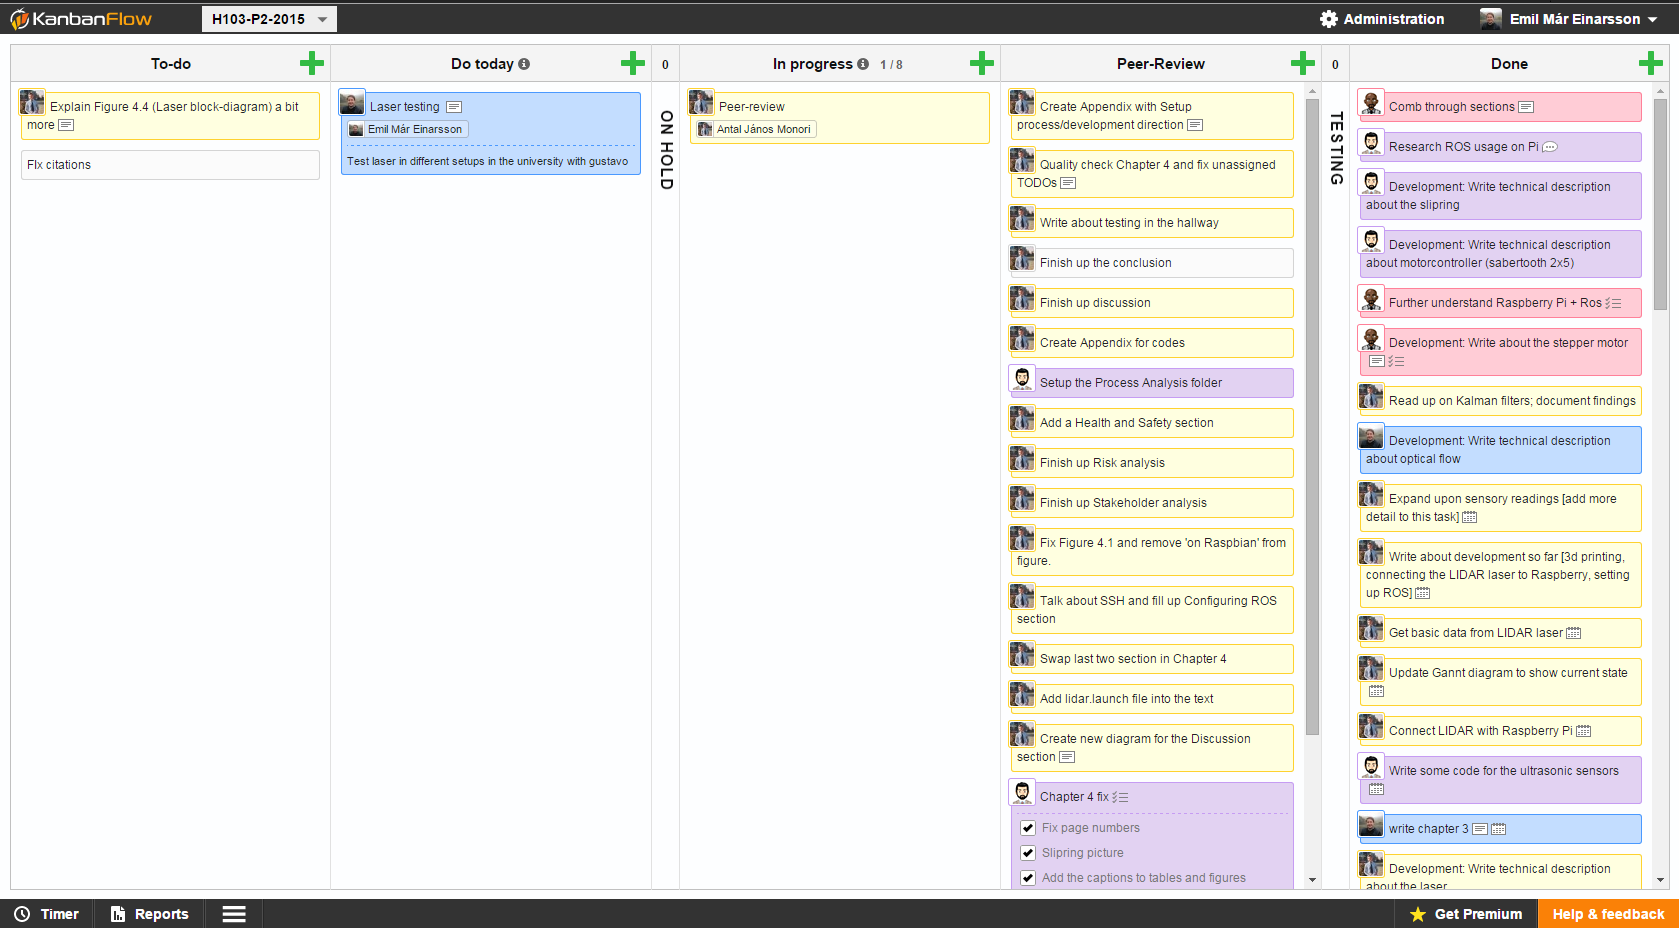
\includegraphics[width=1\linewidth]{images/kanban.png}
	\caption{Screenshot from online kanbanflow.}
	\label{fig:kanban}
\end{figure}

\clearpage
\section{Group contract}\label{appendix:group-contract}

\begin{enumerate}
	\item Honesty is expected from everybody.
	\item Deadlines must be communicated up front, visualized and kept in mind during the whole project period.
	\item Postponing deadlines must be communicated at least halfway through the progress.
	\item During each meeting, deadlines must be set and followed up on.
	\item If the deadlines are not met, it will be brought up at the next strategy meeting.
	\item We aim to work at our full potential and get an acceptable grade, 7.
	\item All members take personal responsibility in achieving the learning goals, but it is expected.
	\item We keep all communications in English.
	\item We must notify each other when running late prior to the start of a meeting. Any notification after a meeting's start time is not taken into consideration.
	\item Wait time for late runners is 10 minutes maximum, with reasonable motive, otherwise we carry on without the missing participant(s).
	\item We penalize late runners or group members who do not comply with any of the following agreements:
	\begin{itemize}
		\item First strike: Warning + Reimbursement in form of beverages for all group members
		\item Second strike: Serious conversation within the team
		\item Third strike: Bringing the issue to our supervisor's attention
	\end{itemize}
	
	\item Attending the report writing meetings is not compulsory, but recommended. A 12-hour notice is required in case you can not attend one of them. Sickness is excluded from this rule.
	\item Skype calls can be used, in case a person is missing a meeting or a report writing session.
	\item The opportunity shall be given to everybody to speak up and raise their concerns in each and every topic of discussion.
	\item When there is a disagreement in a discussion there needs to be an underlining argument.
	\item Leave no junk behind in the meeting rooms before leaving.
	\item We must accept each others interests in regards of attending scheduled classes and courses.
	\item Major problems within the group shall be solved in collaboration with the supervisor.
	\item Everybody is expected to participate in the project with equal amount of work.
	\item We must respect each others work methods and need for breaks (within reasonable boundaries).
	\item The group contract needs to be reviewed by the 1st of April, 2015.
	\item We expect the group members to take their own initiative and self-assignment when there are no delegated tasks.
	\item We do not schedule work meetings.
	\item In the start of the strategy meeting, we read up the agenda and announce the note-taker for the meeting.
	\item We expect everybody to be responsible for adding their own tasks to the online Kanban board and to keep track of it.
	\item We only move tasks to the Done column on the online Kanban board, after it has been reviewed during a strategy meeting.
\end{enumerate}

\textit{In the section below, the members of the group will sign the following statement, acknowledging the agreements above and understanding the consequences in case any of them will be broken.}

\textit{Hereby, I confirm by signing this document, that I will comply to all the rules agreed in this contract. I will make sure that all the other team members does the same, and will raise awareness if I will learn about a misconduct within the group.}

Signed by:

@anthonymonori, @utommo, @42f87d89, @emilioamores

The validity of this contract runs for the period of the P1 project, in the timeframe of 02.02.2012 - 28.06.2015
